% !TEX root = ../Vorlage_DA.tex
%	########################################################
% 					Autoren
%	########################################################


%	--------------------------------------------------------
% 	Überschrift, Inhaltsverzeichnis
%	--------------------------------------------------------
\chapter*{Authors} \markboth{Authors}{Authors}
\addcontentsline{toc}{chapter}{Authors}

%	--------------------------------------------------------
% 	Autor 1
%	--------------------------------------------------------
\htlParagraph{Alexander Voglsperger}

\renewcommand{\arraystretch}{1.2}
\begin{tabularx}{1\textwidth}{@{} l X l @{}}

\emph{Birthday, Place of birth:} & 25.03.2001, Ried im Innkreis & 
\multirow{5}{2.5cm}{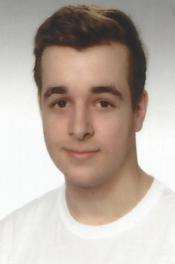
\includegraphics[width=2.5cm]{./media/images/alexander.png}
} 
\\
\emph{School education:} & Volksschule Aurolzmünster \newline Informatik Hauptschule Aurolzmünster \newline HTL Braunau & \\
\emph{Internship:} & Team7 Natürlich Wohnen GmbH, 4 Weeks, IT\newline
Krankenhaus Ried im Innkreis, 4 Weeks, IT\newline
Johannes Kepler University - AI Lab, 4 Weeks, Mapping and Tracking on self-driving car&\\
\emph{Address:} & Forchtenau 196\newline 4971, Aurolzmünster\newline Österreich & \\
\emph{E-Mail:} & alexander.voglsperger@gmail.com & \\

\end{tabularx}
\\\\

%	--------------------------------------------------------
% 	Autor 2
%	--------------------------------------------------------
\htlParagraph{Simon Moharitsch}

\begin{tabularx}{1\textwidth}{@{} l X l @{}}
\emph{Birthday, Place of birth:} & 01.01.1970, Braunau am Inn & 
\multirow{5}{2.5cm}{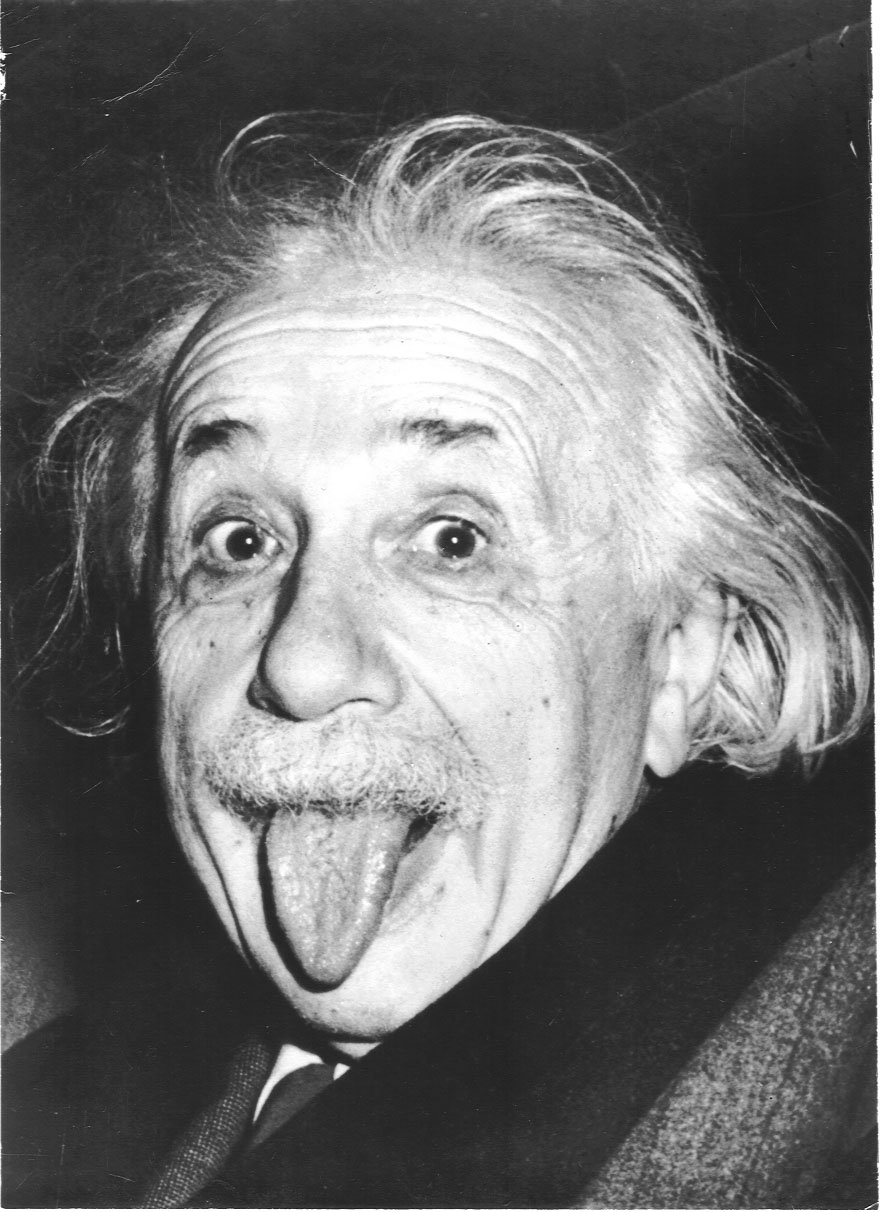
\includegraphics[width=2.5cm]{./media/images/einstein.jpg}
} 
\\
\emph{School education:} & Volksschule \newline Hauptschule \newline HTL & \\
\emph{Internship:} & Firmenname, Zeit, Tätigkeit & \\
\emph{Address:} & Strasse Nummer\newline PLZ, Ort\newline Österreich & \\
\emph{E-Mail:} & max@mustermann.com & \\

\end{tabularx}
